\chapter{SMTP: Simple Mail Transfer Protocol}

\section{Introduction}
The Simple Mail Transfer Protocol (SMTP) is a protocol for sending emails in an
IP network. It can be used between an email client and an outgoing mail server
or between two SMTP servers. SMTP is often combined with the IMAP or POP3
protocols, which can fetch emails and send emails. In principle, it is a
client-server-based protocol, although SMTP can be used between a client and a
server and between two SMTP servers. In this case, a server effectively acts as
a client.

The original SMTP protocol supported only unauthenticated unencrypted 7-bit
ASCII text communications, susceptible to trivial man-in-the-middle attack,
spoofing, and spamming, and requiring any binary data to be encoded to readable
text before transmission. Due to absence of a proper authentication mechanism,
by design every SMTP server was an open mail relay.

An {\bf open mail relay} is a SMTP server configured in such a way that it
allows anyone on the Internet to send e-mail through it, not just mail destined
to or originating from known users.

In November 1995, RFC 1869 defined {\bf Extended Simple Mail Transfer Protocol
    (ESMTP)}, which established a general structure for all existing and future
    extensions which aimed to add-in the features missing from the original
    SMTP. ESMTP defines consistent and manageable means by which ESMTP clients
    and servers can be identified and servers can indicate supported
    extensions. 

Message submission (RFC 2476) and
\href{https://en.wikipedia.org/wiki/SMTP_Authenticatio}{SMTP-AUTH
(RFC 2554)} were introduced in 1998
and 1999, both describing new trends in email delivery. Originally, SMTP
servers were typically internal to an organization, receiving mail for the
organization from the outside, and relaying messages from the organization to
the outside. But as time went on, SMTP servers ({\bf mail transfer agents MTA}), in
practice, were expanding their roles to become {\bf message submission agents
(MSA)}for {\bf Mail user agents (MUA)}, some of which were now relaying mail
from the outside of an organization. (e.g. a company executive wishes to send
email while on a trip using the corporate SMTP server.) 

A  {\bf MSA} is a computer program or software agent that receives electronic
mail messages from a mail user agent (MUA) and cooperates with a mail transfer
agent (MTA) for delivery of the mail. It uses ESMTP. both MTA and MSA functions
use port number 25, but the official port for MSAs is 587.The MTA accepts a
user's incoming mail, while the MSA accepts a user's outgoing mail. 

This issue, a consequence of the rapid expansion and popularity of the World
Wide Web, meant that SMTP had to include specific rules and methods for
relaying mail and authenticating users to prevent abuses such as relaying of
unsolicited email (spam). Work on message submission (RFC 2476) was originally
started because popular mail servers would often rewrite mail in an attempt to
fix problems in it, for example, adding a domain name to an unqualified
address. This behavior is helpful when the message being fixed is an initial
submission, but dangerous and harmful when the message originated elsewhere and
is being relayed. Cleanly separating mail into submission and relay was seen as
a way to permit and encourage rewriting submissions while prohibiting rewriting
relay. As spam became more prevalent, it was also seen as a way to provide
authorization for mail being sent out from an organization, as well as
traceability. This separation of relay and submission quickly became a
foundation for modern email security practices. 

As this protocol started out purely ASCII text-based, it did not deal well with
binary files, or characters in many non-English languages. Standards such as
Multipurpose Internet Mail Extensions (MIME) were developed to encode binary
files for transfer through SMTP. 

\subsection{Mail processing model}


\begin{figure}
  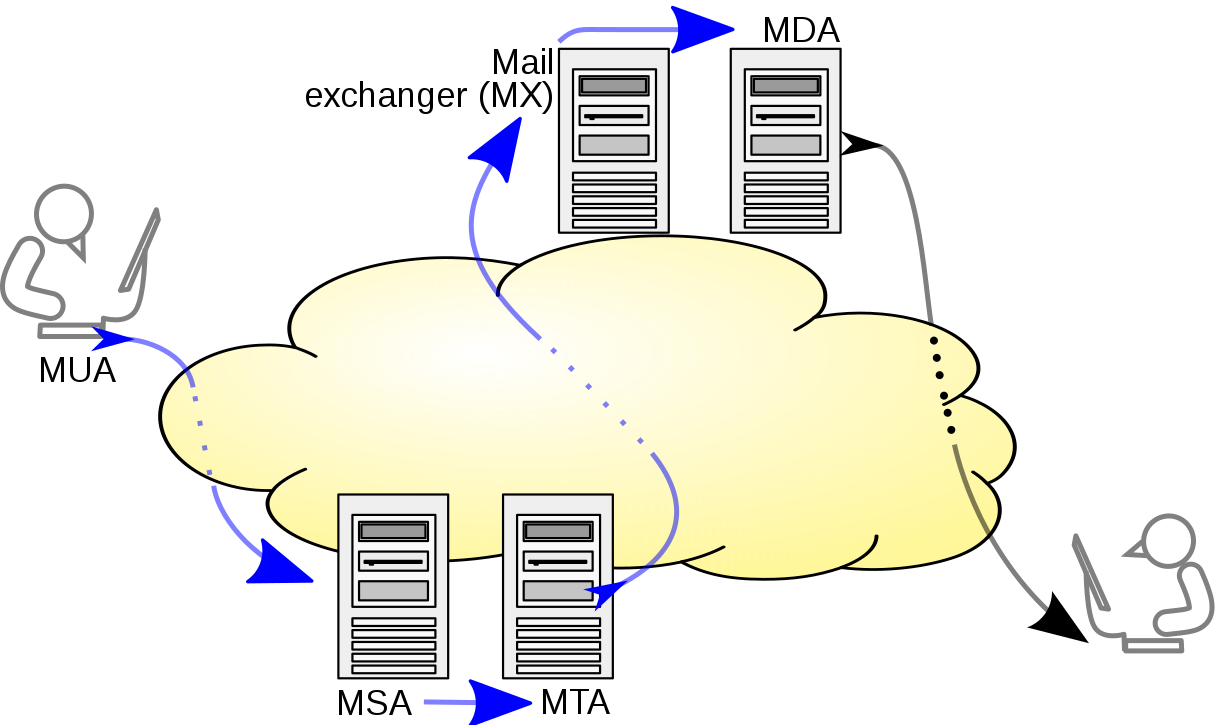
\includegraphics[width=\linewidth]{network/smtp/images/SMTP-transfer-model.png}
  \caption{SMTP transfer model}
  \label{fig:smtp-transfer-model}
\end{figure}

Email is submitted by a MUA to a mail server MSA using SMTP on TCP port 587.
Most mailbox providers still allow submission on traditional port 25. The MSA
delivers the mail to its MTA. Often, these two agents are instances of the same
software launched with different options on the same machine. If processing is
on multiple machines, they transfer messages between each other using SMTP,
where each machine is configured to use the next machine as a smart host. Each
process is an MTA (an SMTP server) in its own right. 

The boundary MTA uses DNS to look up the MX (mail exchanger) record for the
recipient's domain. The MX record contains the name of the target MTA. Based on
the target host and other factors, the sending MTA selects a recipient server
and connects to it to complete the mail exchange.

Message transfer can occur in a single connection between two MTAs, or in a
series of hops through intermediary systems. A receiving SMTP server may be the
ultimate destination, an intermediate "relay" (that is, it stores and forwards
the message) or a "gateway" (that is, it may forward the message using some
protocol other than SMTP).

Once the final hop accepts the incoming message, it hands it to a {\bf mail
delivery agent (MDA)} for local delivery. An MDA saves messages in the relevant
mailbox format. As with sending, this reception can be done using one or
multiple computers, but in the diagram above the MDA is depicted as one box
near the mail exchanger box. An MDA may deliver messages directly to storage,
or forward them over a network using SMTP or other protocol such as
\href{https://en.wikipedia.org/wiki/Local_Mail_Transfer_Protocol}{Local Mail
Transfer Protocol (LMTP)}, a derivative of SMTP designed for this purpose.

SMTP defines message transport, not the message content. Thus, it defines the
mail envelope and its parameters, such as the envelope sender, but not the
header (except trace information) nor the body of the message itself. STD 10
and \href{https://datatracker.ietf.org/doc/html/rfc5321}{RFC 5321} define SMTP
(the envelope), while STD 11 and
\href{https://datatracker.ietf.org/doc/html/rfc5322}{RFC5322} define the
message (header and body), formally referred to as the Internet Message
Format.

\subsection{SMTP commands and example}

The sending and communication are also done by special commands that cause the
SMTP server to do what the user requires.
\begin{itemize}
    \item Basic SMTP commands:
        \begin{itemize}
            \item \verb+HELO domain+: logs in with its computer name and thus starts
    the session.
            \item \verb+MAIL FROM+: names the email sender.
            \item \verb+RCPT TO+: names the email recipient.
            \item \verb+DATA+: initiates the transmission of the email.
            \item \verb+RSET+: aborts the initiated transmission but keeps the connection between client and server.
            \item \verb+NOOP+: requests a response from the server to prevent disconnection due to time-out.
            \item \verb+QUIT+: terminates the session.
        \end{itemize}
    \item Extended SMTP (ESMTP) Commands:
        \begin{itemize}
            \item \verb+EHLO+: initiates the SMTP communication
            \item \verb+AUTH method+: used to authenticate the client to the
                server (\verb+PLAIN+, \verb+NTLM+, \verb+CRAM-MD5+,
                \verb+DIGEST-MD5+,\ldots)
            \item \verb+VRFY+: checks if a mailbox is available for message transfer.
            \item \verb+EXPN+: checks if a mailbox is available for messaging with this command.
            \item \verb+STARTTLS+: 
            \item \verb+HELP+ 	Help.
        \end{itemize}
\end{itemize}

\begin{verbatim}
telnet IP 25
EHLO inlanefreight.htb

250-mail1.inlanefreight.htb
250-PIPELINING
250-SIZE 10240000
250-ETRN
250-ENHANCEDSTATUSCODES
250-8BITMIME
250-DSN
250-SMTPUTF8
250 CHUNKING


MAIL FROM: <cry0l1t3@inlanefreight.htb>
250 2.1.0 Ok
RCPT TO: <mrb3n@inlanefreight.htb> NOTIFY=success,failure
250 2.1.5 Ok
DATA
354 End data with <CR><LF>.<CR><LF>
From: <cry0l1t3@inlanefreight.htb>
To: <mrb3n@inlanefreight.htb>
Subject: DB
Date: Tue, 28 Sept 2021 16:32:51 +0200
Hey man, I am trying to access our XY-DB but the creds don't work.
Did you make any changes there?
.

250 2.0.0 Ok: queued as 6E1CF1681AB
QUIT
221 2.0.0 Bye
Connection closed by foreign host.
\end{verbatim}


\subsection{SMTP Extensions}
\subsection{Extension discovery mechanism}

Clients learn a server's supported options by using the \verb+EHLO+ greeting, as
exemplified below, instead of the original \verb+HELO+. Clients fall back to
\verb+HELO+ only if the server does not support EHLO greeting.

Modern clients may use the ESMTP extension keyword SIZE to query the server for
the maximum message size that will be accepted. Older clients and servers may
try to transfer excessively sized messages that will be rejected after
consuming network resources, including connect time to network links that is
paid by the minute.

Users can manually determine in advance the maximum size accepted by ESMTP
servers. The client replaces the HELO command with the EHLO command.

\begin{verbatim}
$ telnet 10.10.11.175 25
Trying 10.10.11.175...
Connected to 10.10.11.175.
Escape character is '^]'.
220 mail.outdated.htb ESMTP
EHLO outdated.htb
250-mail.outdated.htb
250-SIZE 20480000
250-AUTH LOGIN
250 HELP
\end{verbatim}

\subsubsection{STARTTLS or "Opportunistic TLS}
The STARTTLS extensions enables supporting SMTP servers to notify connecting
clients that it supports TLS encrypted communication and offers the opportunity
for clients to upgrade their connection by sending the STARTTLS command.
Servers supporting the extension do not inherently gain any security benefits
from its implementation on its own, as upgrading to a TLS encrypted session is
dependent on the connecting client deciding to exercise this option, hence the
term opportunistic TLS.

By sending {\bf STARTTLS}  after the {\bf EHLO command} the communication is
switched on port  465.

\begin{verbatim}
openssl s_client -crlf -connect smtp.mailgun.org:465 #SSL/TLS without starttls 
openssl s_client -starttls smtp -crlf -connect smtp.mailgun.org:587
\end{verbatim}

\section{Dangerous Settings}
To prevent the sent emails from being filtered by spam filters and not reaching
the recipient, the sender can use a relay server that the recipient trusts. It
is an SMTP server that is known and verified by all others. As a rule, the
sender must authenticate himself to the relay server before using it.

Often, administrators have no overview of which IP ranges they have to allow.
This results in a misconfiguration of the SMTP server that we will still often
find in external and internal penetration tests. Therefore, they allow all IP
addresses not to cause errors in the email traffic and thus not to disturb or
unintentionally interrupt the communication with potential and current
customers.


\section{Footprint / enumeration}

\subsection{nmap}

\begin{verbatim}
sudo nmap -p25 --script smtp-commands -v
sudo nmap -p25 --script smtp-open-relay -v
sudo nmap -p25 --script smtp-enum-users -v
\end{verbatim}

\begin{itemize}
    \item
        \href{https://nmap.org/nsedoc/scripts/smtp-enum-users.html}{smtp-enum-users.nse}:
        attempts to enumerate the users on a SMTP server by issuing the VRFY,
        EXPN or RCPT TO commands. Arguments:
        \begin{itemize}
            \item smtp.domain:
            \item smtp-enum-users.methods
            \item passdb, unpwdb.passlimit, unpwdb.timelimit, unpwdb.userlimit,
                userdb: See the documentation for the
                \href{https://nmap.org/nsedoc/lib/unpwdb.html#script-args}{unpwdb
                library}.
            \item smbdomain, smbhash, smbnoguest, smbpassword, smbtype,
                smbusername: See the documentation for the
                \href{https://nmap.org/nsedoc/lib/smbauth.html#script-args}{smbauth} library.
        \end{itemize}
    \item \verb+smtp-open-relay+ identify the target SMTP server as an open
        relay using 16 different tests.
\end{itemize}

\subsection{metasploit}
\begin{verbatim}
use auxiliary/scanner/smtp/smtp_enum
use auxiliary/scanner/smtp/smtp_relay
\end{verbatim}

\subsection{smtp-user-enum}
s 3 methods of user enumeration.The commands that this tool is using in order
to verify usernames are the EXPN,VRFY and RCPT.It can also support single
username enumeration and multiple by checking through a .txt list.

The mail header is the carrier of a large amount of interesting information in
an email. Among other things, it provides information about the sender and
recipient, the time of sending and arrival, the stations the email passed on
its way, the content and format of the message, and the sender and recipient.

Some of this information is mandatory, such as sender information and when the
email was created. Other information is optional. However, the email header
does not contain any information necessary for technical delivery. It is
transmitted as part of the transmission protocol. Both sender and recipient can
access the header of an email, although it is not visible at first glance. The
structure of an email header is defined by
\href{https://datatracker.ietf.org/doc/html/rfc5322}{RFC5322}.



\section{Open Relay}
An open relay is a Simple Transfer Mail Protocol server, which is
improperly configured and allows an unauthenticated email relay. Messaging
servers that are accidentally or intentionally configured as open relays allow
mail from any source to be transparently re-routed through the open relay
server. This behavior masks the source of the messages and makes it look like
the mail originated from the open relay server.

From an attacker's standpoint, we can abuse this for phishing by sending emails
as non-existing users or spoofing someone else's email. For example, imagine we
are targeting an enterprise with an open relay mail server, and we identify
they use a specific email address to send notifications to their employees. We
can send a similar email using the same address and add our phishing link with
this information. With the nmap smtp-open-relay script, we can identify if an
SMTP port allows an open relay.

\begin{verbatim}
nmap -p25 -Pn --script smtp-open-relay 
\end{verbatim}

\section{Mail spoofing}
Most of this section was extracted from the book {\bf Network Security
Assessment 3rd Edition.}

SMTP messages are easily spoofed, and so organizations use SPF, DKIM, and DMARC
features to prevent parties from sending unauthorised email.

A complete guide of these countermeasures can be found in
\url{https://seanthegeek.net/459/demystifying-dmarc/}

\subsection{Countermeasures}

\subsubsection{SPF}
Sender Policy Framework (SPF) provides a mechanism that allows MTAs to check if
a host sending an email is authorized. Then, the organisations can define a
list of authorised mail servers and the MTAs can query for this lists to check
if the email was spoofed or not. In order to define IP addresses/ranges,
domains and others that are allowed to send email on behalf a domain name,
different "Mechanism" cam appear in the SPF registry.

To check the SPF of a domain you can use online tools like:
\url{https://www.kitterman.com/spf/validate.html}

\subsubsection{DKIM}
DomainKeys Identified Mail (DKIM) is a mechanism by which outbound email is
signed and validated by foreign MTAs upon retrieving a domain’s public key via
DNS. The DKIM public key is held within a TXT record for a domain; however, you
must know both the selector and domain name to retrieve it.

Then, to ask for the key you need the domain name and the selector of the mail
from the mail header 
\begin{verbatim}
dig 20120113._domainkey.gmail.com TXT | grep p=
20120113._domainkey.gmail.com. 280 IN   TXT    "k=rsa\; p=MIIBIjANBgkqhkiG9w0BAQEFAAOCAQ8AMIIBCg
KCAQEA1Kd87/UeJjenpabgbFwh+eBCsSTrqmwIYYvywlbhbqoo2DymndFkbjOVIPIldNs/m40KF+yzMn1skyoxcTUGCQs8g3
\end{verbatim}

\subsubsection{DMARC}
Domain-based Message Authentication, Reporting \& Conformance (DMARC) is a
method of mail authentication that expands upon SPF and DKIM. Policies instruct
mail servers how to process email for a given domain and report upon actions
performed.


\subsection{Tools}

Check for SPF and DMARC misconfigurations:
\url{https://github.com/serain/mailspoof}

Automatically get SPF and DMARC configs:
\url{https://pypi.org/project/checkdmarc/}

You can attack some characteristics of mail clients to make the user think that
the mail is coming from any address, more info:
\url{https://www.mailsploit.com/index}

\url{https://emkei.cz/} can be used to send you an email spoofing an address
and check if reaches you email.
